\setchapterabstract{Lorem ipsum dolor sit amet, consectetur adipiscing elit. Suspendisse augue est, porttitor commodo velit a, tristique pharetra ante. Mauris pretium ante at lorem suscipit porttitor. Sed neque tortor, lacinia a aliquam quis, molestie tincidunt nisi. Vivamus congue cursus iaculis. Aenean id massa convallis, sodales metus a, imperdiet velit. In metus erat, suscipit vel mollis sed, tincidunt at ante. In hac habitasse platea dictumst. Cras malesuada mollis odio, eget mattis mauris tincidunt a.}
\chapter{Probability}
\vspace{-1.5cm}

{\chaptoc\noindent\begin{minipage}[inner sep=0,outer sep=0]{0.9\linewidth}\section{Elementary Probability}\end{minipage}}

        \subsubsection{Permutation}

        \Definition{
        any alignment in $n$ places
                    \begin{equation}
                        P_n = n!
                    \end{equation}
        }{Permutation}

        \subsubsection{Disposition}

        \Definition{
        Any alignment in $k$ places
        \begin{enumerate}
                        \item \textbf{Simple}:
                            \begin{equation}
                                D_{n,k} = n \cdot (n-1) \cdot \cdots \cdot (n-k-1) = \frac{n!}{(n-k)!}
                            \end{equation}
                        \item \textbf{With repetition}:
                            \begin{equation}
                                D_{n,k}^* = n \cdot n \cdot \cdots \cdot n = n^k 
                            \end{equation}
                    \end{enumerate}
        }{Disposition}

        \subsubsection{Combination}

        \Definition{
        any alignment of $k$ objects from $n$
                    \begin{equation}
                        C_{n,k} = \frac{n!}{k!(n-k)!} = \binom{n}{k}
                    \end{equation}
        }{Combination}

\section{Conditional Probability}

    In the probability space \( ( \Omega, A, \mathbb{P}) \), conditional probability can be written as

    \begin{equation}
        \mathbb{P} (E|F) = \frac{\mathbb{P} (E \cap F)}{\mathbb{P} (F)}
    \end{equation}

    \noindent
    with \(\mathbb{P} (F) > 0\)

        \subsubsection{Conditional Probability as Intersection of Events}

            \begin{equation}
            \begin{split}
                \mathbb{P} (E \cap F) = & \mathbb{P} (F) \cdot \mathbb{P} (E | F) \\
                \mathbb{P} (E_1 \cap E_2 \cap \cdots \cap E_n ) = & \mathbb{P} (E_1) \cdot \mathbb{P} (E_2 | E_1) \cdot \mathbb{P} (E_3 | E_2 \cap E_1) \cdots \mathbb{P} (E_n | E_1 \cap E_2 \cap \cdots \cap E_{n-1})
            \end{split}
            \end{equation}

        \subsubsection{Law of Total Probability}

            Given \(E_1, \ E_2, \ \cdots \ E_n\) partitions of \(\Omega\) and the conditions

            \begin{enumerate}
                \item \(E_i \cap E_j = \emptyset \forall i \neq j\)
                \item \(E_1 \cup E_2 \cup \cdots \cup E_n = \Omega\)
            \end{enumerate}

            \noindent
            We can state that:

            \begin{equation}
                \mathbb{P} (F) = \sum^{n}_{i=1} \mathbb{P} (F|Ei) \mathbb{P} (E_i)
            \end{equation}

        \subsubsection{Bayes Formula}

            Given 

            \begin{equation}
                \mathbb{P} (E_n | F) = \frac{\mathbb{P} (F| E_n) \mathbb{P} (E_n)}{\sum^{n}_{i=1} \mathbb{P} (F|Ei) \mathbb{P} (E_i)} \rightarrow \mathbb{P} (A|P) \frac{\mathbb{P} (B|A) \mathbb{P} (A)}{\mathbb{P} (B)}
            \end{equation}

\section{Independent Events}

        \subsubsection{Stochastic Independence}

            \Definition{
            Given the probability space \( ( \Omega, A, \mathbb{P} ) \), two events \(E, F \in A\) are said to be \textbf{stocastically independent} if \(\mathbb{P} (E) \cap \mathbb{P} (F) = \mathbb{P} (E) \cdot \mathbb{P} (F)\)
            \begin{equation}
                \mathbb{P} (E|F) = \mathbb{P} (E) \iff \mathbb{P} (F|E) = \mathbb{P} (F)
            \end{equation}
            }{Stochastic Independence}
            

        \subsubsection{Conditional Stochastic Independence}

            \Definition{
            Given the probability space \( ( \Omega, A, \mathbb{P} ) \) and the events \(A, B, F \), \textbf{Conditional Stochastic Independence} can be characterised as:
            \begin{equation}
                \mathbb{P} (A \cap B | F) = \mathbb{P} (A|F) \cdot \mathbb{P} (B|F)
            \end{equation}
            }{Conditional Stochastic Independence}

            \Warning{
            Stochastic Independence \textbf{does not imply} Conditional Stochastic Independence, and vice versa.
            }
            

\section{Random Variables}

        Given the sample space of tossing a dice \(\Omega = \{1,2,3,4,5,6\} \), we can define:

            \[X: \Omega \rightarrow \mathbb{R} \]

        \Remark{
        In the equation above:
                \begin{itemize}
                    \item if \(\Omega\) is finite \(\rightarrow\) it is a random variable
                    \item if \(\Omega\) is discrete \(\rightarrow\) it is \textbf{not} a random variable 
                \end{itemize}
        }

        \noindent
        Properties to be considered a random variable:

            \begin{itemize}
                \item \(\forall t \in \mathbb{R}\)

                    \( \{ \omega \in \Omega : X (\omega) \leq t \} = E_t \in A \)

                    With \(X\) being \textbf{Borel measurable}

                \item 

                    \( \mathbb{P} (E_t) = \mathbb{P} (\omega \in \Omega : X (\omega) \leq t ) = \mathbb{P} (X (\omega) \leq t) = \mathbb{P} (X \leq t)  0 F_x (t)  \)
 
                \item \(F_x : \mathbb{R} \rightarrow \mathbb{R}\), with \(F_x(t)\) being the distribution function of the variable.

                    \( \lim _{t \to - \infty} F(t) = 0 \)    

                    \( \lim _{t\to\infty} F(t) = 1\)

                    \begin{itemize}
                        \item If \(X\) is discrete, the graph will possess the following properties:
                            \begin{enumerate}
                                \item Stepwise
                                \item Non-decreasing 
                                \item \(F_x\) continuous from the right
                            \end{enumerate}
                        \item If \(X\) is \textcolor{dblue}{absolutely} continuous
                            \begin{enumerate}
                                \item \(F\) is continuous
                            \end{enumerate}
                    \end{itemize}
            \end{itemize}

            \begin{figure}[h]
                \centering
                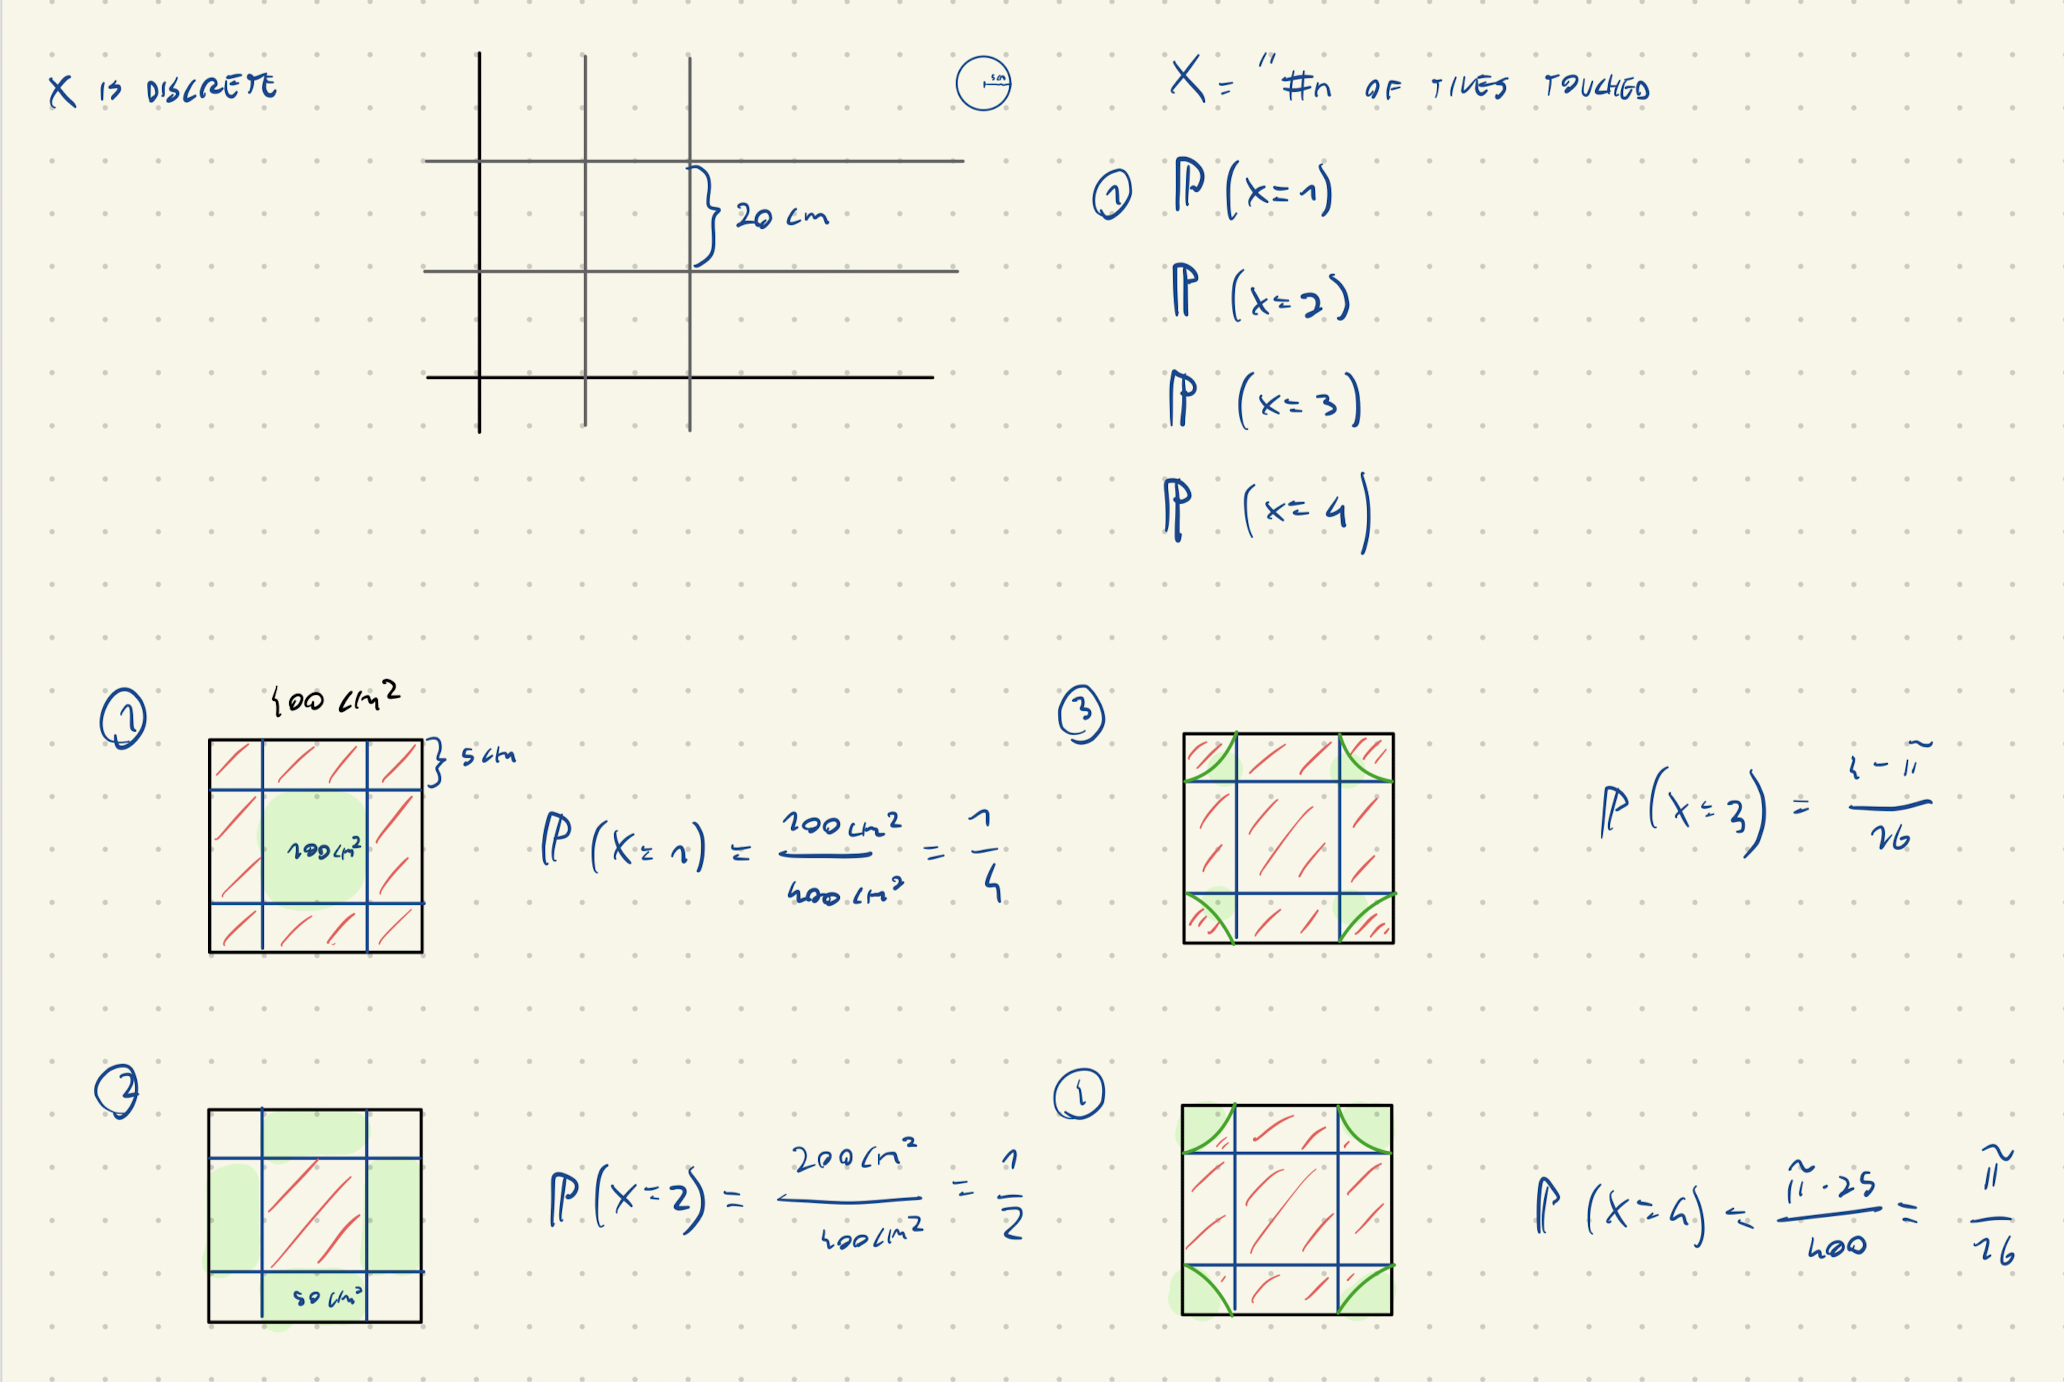
\includegraphics[width=0.90\linewidth]{X_visual_discrete.png}
                \caption{Visual representation of an example where \(X\) is a \textbf{discrete} random variable}
                \label{fig:X_visual_discrete}
            \end{figure}

            \begin{figure}[h]
                \centering
                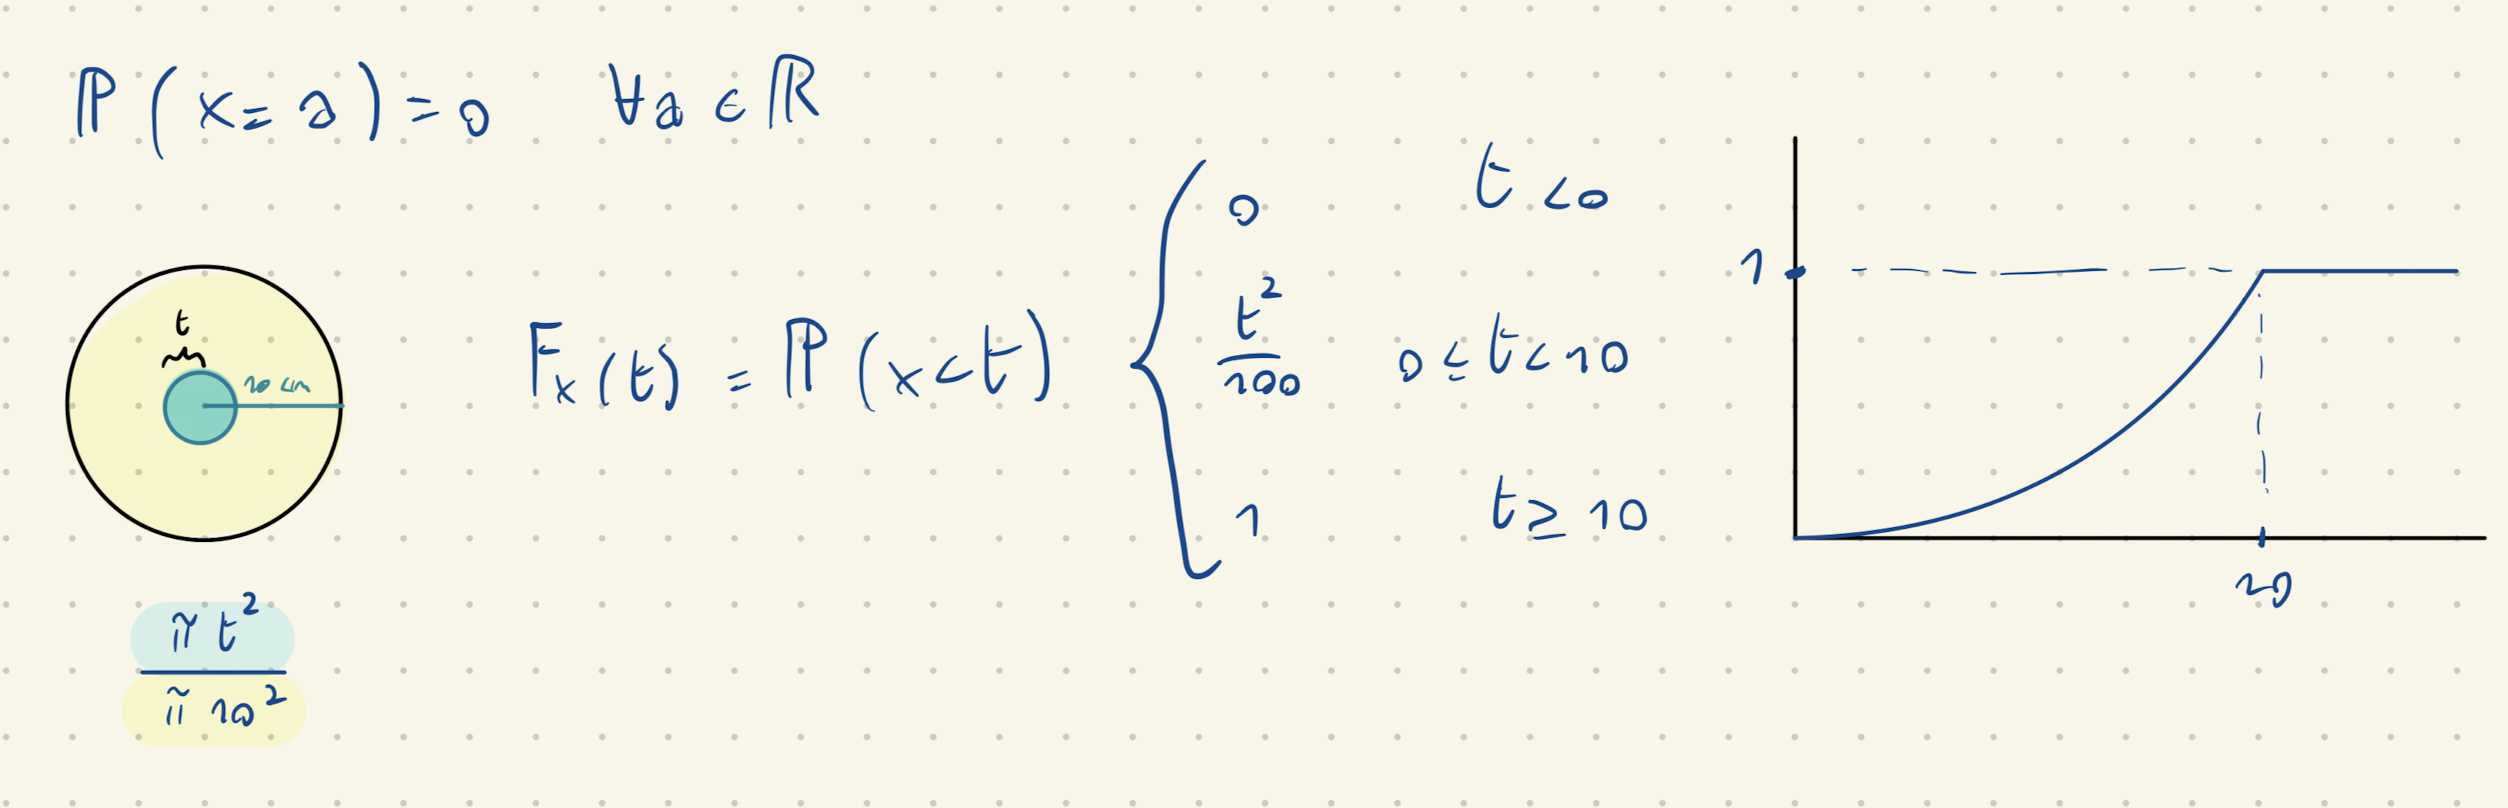
\includegraphics[width=0.90\linewidth]{X_visual_absolutely_continuous.png}
                \caption{Visual representation of an example where \(X\) is an \textbf{absolutely continuous} random variable}
                \label{fig:X_visual_absolutely_continuous}
            \end{figure}